We first describe our solution for generating automated reasoning
benchmarks in a fully automated and random manner. We used this
setting to generate exam problems on SAT solving and first-order
theorem proving by filtering out problem instances that are either too
hard or too easy. Throughout this paper, we assume basic familiarity with standard first-order
logic and refer to the literature~\cite{SAT09,Vampire13} for further details.


\subsection{Boolean Satisfiability (SAT)}\label{sec:sat}

In our exam problem on SAT solving (Problem 1 of Figure~\ref{fig:exam}), students were asked to
(a)~determine which atoms are of pure polarity in the formula,
(b)~compute a polarity-optimized clausal normal form (CNF)~\cite{Tseytin70},
and (c)~decide satisfiability of the computed CNF formula by applying the DPLL algorithm.

Randomly generating propositional formulas in a naive setting would lead
to a huge variety of formulas,
spanning both formulas for which the above questions %on SAT solving
are trivial to answer (e.g., clauses as propositional tautologies)
and others requiring much more effort
(e.g., arbitrary formulas using only ``$\leftrightarrow$'').
More work was thus needed to
ensure comparable workload for solving exam sheets.
%This is obviously undesirable in an exam setting,
%where the tasks should ultimately be challenging, but still solvable by hand.
% Further,
% the variation in difficulty between different exams should be kept as small as possible,
% to make the setting as fair to the examinees as possible.

To this end, we identified several  syntactical characteristics
that the exam problems on SAT solving should exhibit,
and filtered the generated formulas by these, as summarized  partially
below.

%
% The criteria are the following:
% Size: 7 connectives
% [ numAtoms fm == 3
% , -- there is at least one atom with pure polarity
%   hasAtomPolarity Neg fm || hasAtomPolarity Pos fm
% , not (anySubformula isNestedNot fm)
% , -- at least one but at most two equivalences
%   let n = countSubformulas isIff fm
%   in 1 <= n && n <= 2
% , anySubformula isImp fm
% , anySubformula isNot fm
% , anySubformula isAnd fm || anySubformula isOr fm
% , not (anySubformula isTrivialBinaryConnective fm)
% , hasVarietyInDefinitionalNF fm
% , length (models fm) <= 6
% , nestedLatexParens fm < 3
% ]

\begin{itemize}
\item[(i)] %\label{item:satsize} %    \item
        The SAT formula contains exactly seven logical connectives 
        and exactly three different propositional variables. \smallskip
        % (but each of these may appear multiple times).
    % \item
    %     The formula contains exactly seven connectives.
    % \item
    %     The formula contains exactly three different atomic propositions
    %     (but each of these may appear multiple times).

\item[(ii)]
%    \item\label{item:polarity}
        There is at least one atom that appears with a pure polarity.\smallskip
        % (i.e., either only in positive position or only in negative
        % position).

\item[(iii)] %\label{item:satconn} %   \item
        The connectives ``$\leftrightarrow$'', ``$\rightarrow$'', and ``$\lnot$'' appear at least once,
        with ``$\leftrightarrow$'' appearing at most twice.
        At least one of ``$\land$'' and ``$\lor$'' appears. \smallskip
    % \item
    %     The connective ``$\leftrightarrow$'' appears at least once but at most twice.
    % \item
    %     The connectives ``$\rightarrow$'' and ``$\lnot$'' appear at least once.
    % \item
    %     At least one of the connectives ``$\land$'' or ``$\lor$''
    %     appears in the formula.
        
%LK commented out these 2
    %   \item
%        There is no subformula for the form $\lnot \lnot \varphi$ for any formula $\varphi$.
%    \item
 %       There are no trivial binary subformulas such as $p \land
 %       \lnot p$ or $p \lor p$.
 %       LK end
        
    % \item
    %     If a binary connective has a literal as argument,
    %     the other argument cannot also be a literal containing the same atomic proposition.
    %     % No binary connective has two literals that contain the same atomic proposition.
    %     % There is no binary connective that
    %     For example, this excludes subformulas such as $p \land \lnot p$ and $p \lor p$,
    %     but not $p \rightarrow q$.

\item[(iv)]
        % The polarity-optimized clausal normal form of the SAT formula should not be trivial.
        % \todo{JR: the first sentence reads like a restriction when it's in fact an explanation}
        Recall that the polarity-optimized clausal normal form involves a set of definitions,
        each of which is of the form
        $n \circ \varphi$ with $\circ \in \{ \rightarrow, \leftarrow, \leftrightarrow \}$,
        a fresh propositional variable~$n$, and a formula~$\varphi$.
        We restrict the SAT formula such that at least two of the choices for
        $\circ$ appear in its CNF.\smallskip

\item[(v)]
        The SAT formula has at most six models.
        % Since there are $2^3 = 8$ different interpretations,
        % this means the formula is not valid.
        \smallskip

% \noindent(6)
%         To avoid accidental difficulty introduced by visual complexity,
%         the \LaTeX{} rendering of the formula should have a parenthesis nesting level of at most two.\smallskip
\end{itemize}

% Of these, items (i) and (iii) were implemented as constraints during formula generation,
% while the other criteria were realized as post-generation filters.

Our aim was to create problems of similar difficulty as in previous iterations of the course,
which is why we used exams from previous years as a reference point.
Some of the criteria, such as the number of connectives and variables,
come from this previous experience.
Other criteria, such as the restrictions on connectives and atom polarity,
have been refined iteratively by checking the output for trivial or too complicated instances.

\begin{figure}
  \makebox[\textwidth][c]{
    % WITHOUT FRAME:
    % 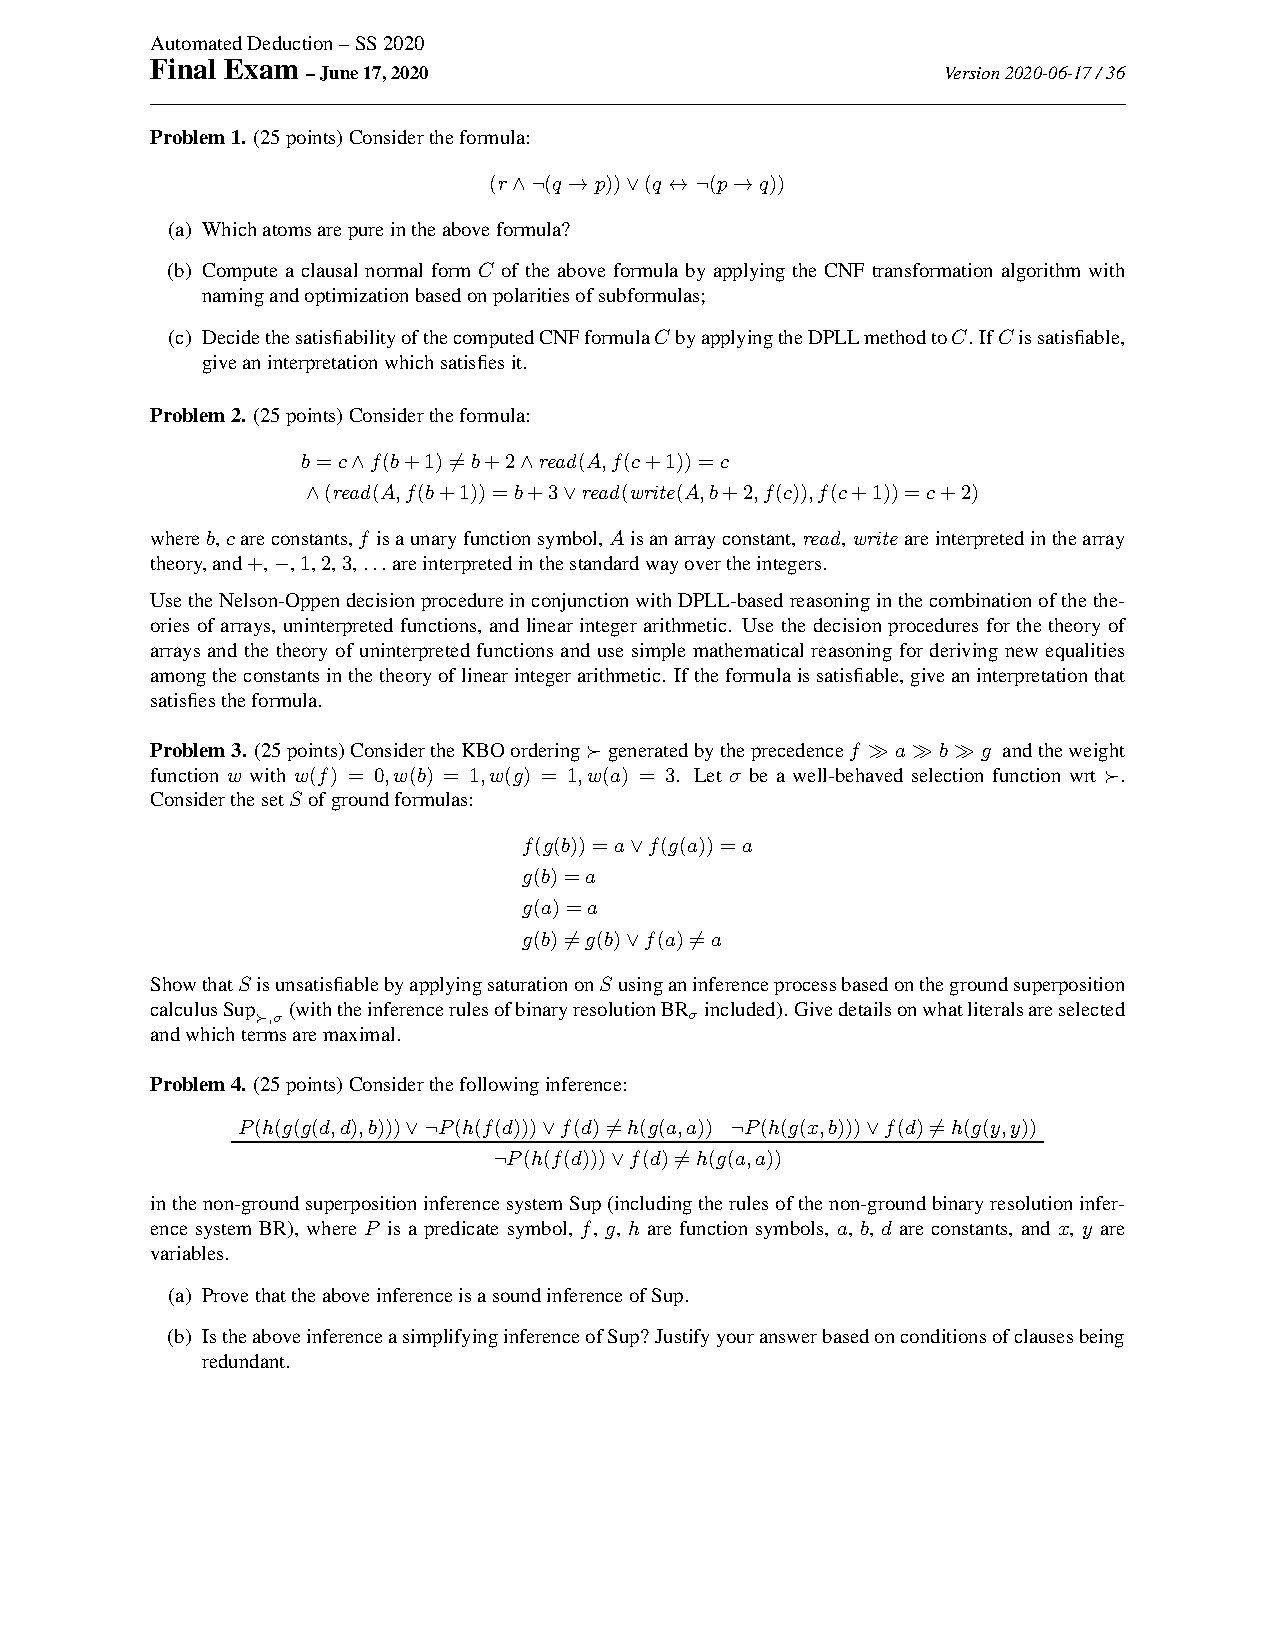
\includegraphics[page=1,width=1.5\textwidth,trim=0in 1.8in 0in 0in]{./exam-36.pdf}
    % WITH FRAME:
    \frame{
      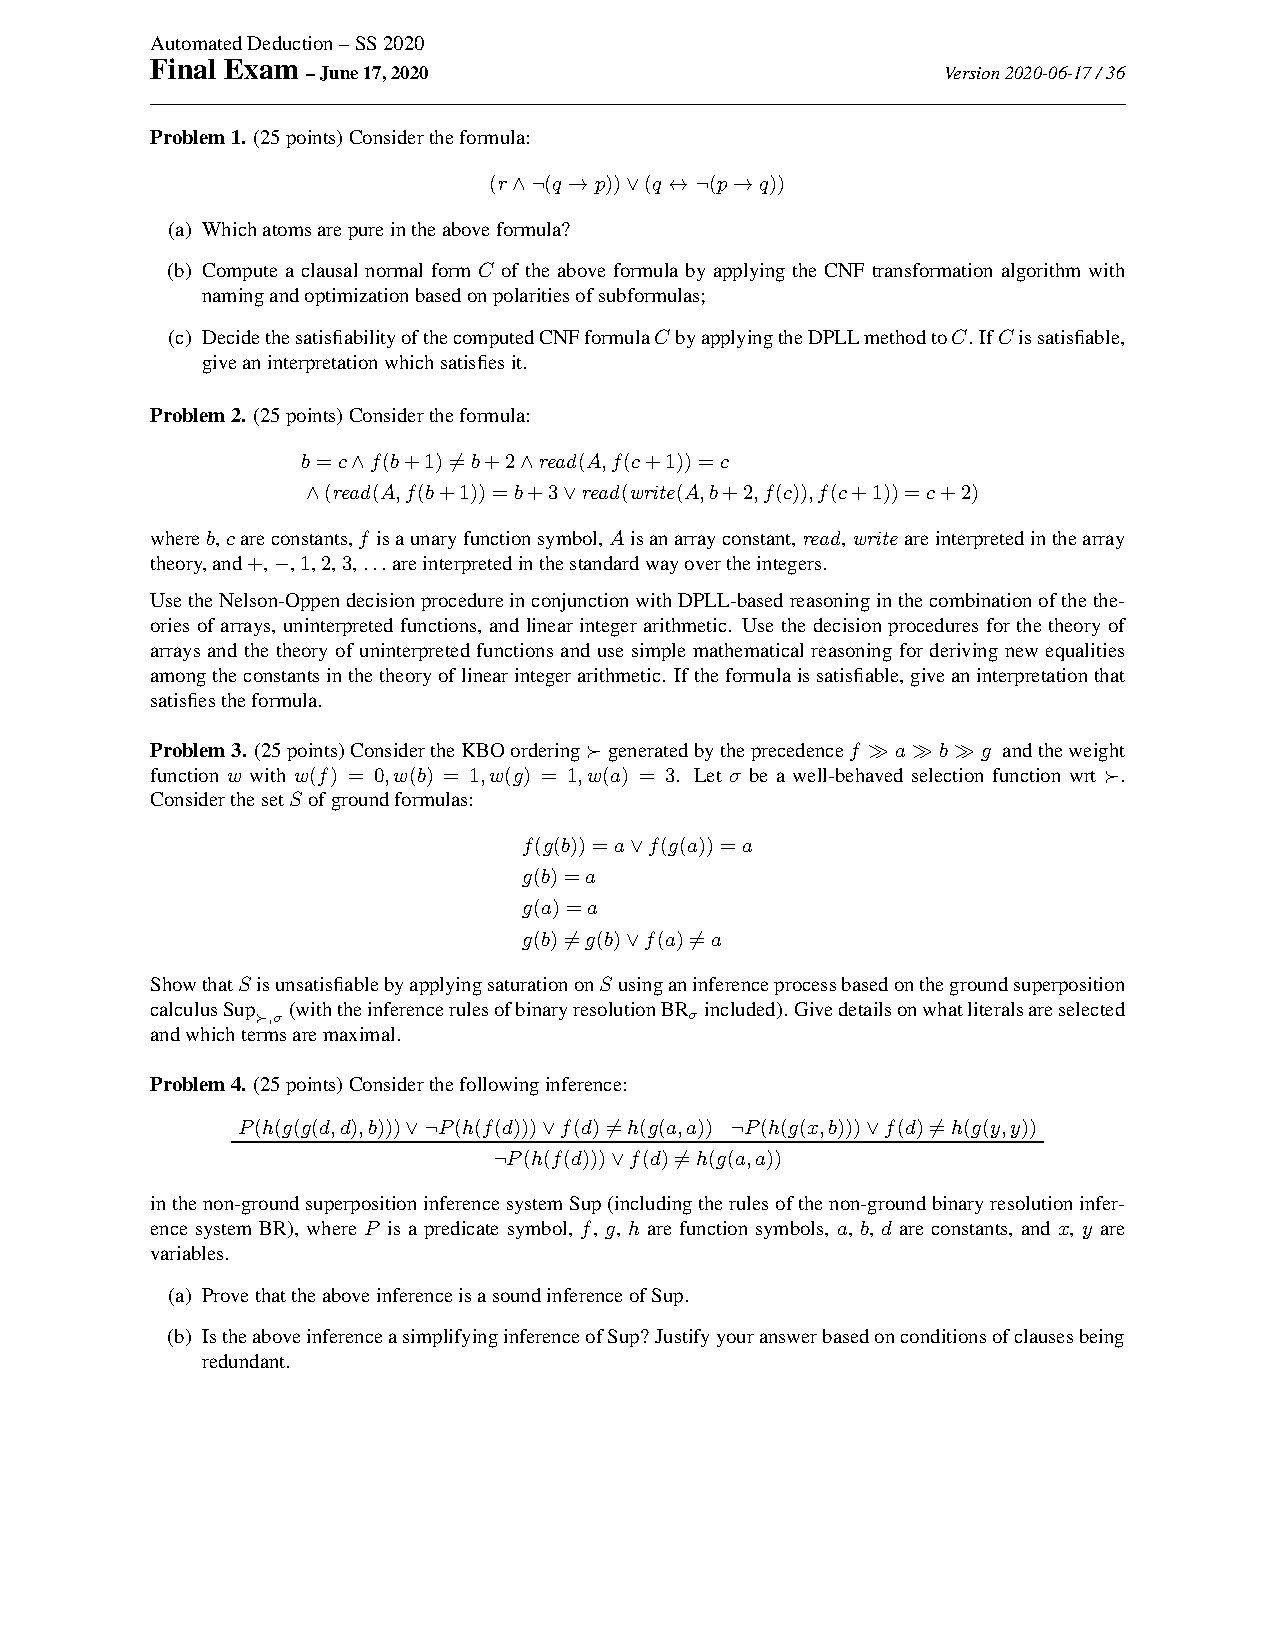
\includegraphics[page=1,width=1.2\textwidth,trim=0.8in 1.7in 0.8in 0.1in]{./exam-36.pdf}
    }
  }
  \caption{An example of a randomly generated exam sheet of automated deduction.}
  \label{fig:exam}
\end{figure}

Although the combination of the above conditions (i)-(v) might seem very restrictive,
we note that 
%Thus, we enumerated the sample space to see how much variety is possible:
%as it turns out,
there are 20\,390\,076 different SAT formulas satisfying the above
criteria.
Further,
if we do not want to distinguish formulas that differ only by a permutation of atoms,
3\,398\,346 formulas remain.
We are thus able to generate a large number of unique SAT formulas to be used in online examinations and
beyond. Problem~1 of Figure~\ref{fig:exam} showcases one SAT
reasoning challenge we automatically generated for one  online
examination sheet. 

We finally note that, while experimenting with the different
constraints (i)-(v) above, we encountered the following
issues that may arise if the restrictions on the randomly generated formula are too strict:
\begin{itemize}
    \item
        The sample space might be empty or very sparse.
        In practice, it seems to the user as if the problem generator got stuck,
        usually resulting in the process being killed by the user.
        For example, consider the restriction on polarities of propositional variables.
        Combined with the other restrictions,
        it is impossible to get a formula that contains atomic propositions
        of purely positive and purely negative polarity at the same time.
    \item
        The second issue manifests less drastically but is perhaps more problematic:
        the sample space may be too uniform,
        leading to the generation of trivial and/or very similar formulas.
        In particular, we encountered this problem
        when we restricted the number of models to exactly one, or zero.
        We note that there simply are not that many ways to rule out eight interpretations
        using only seven connectives.
\end{itemize}





\subsection{Non-Ground Superposition with Redundancy}\label{sec:fo}

Moving beyond Boolean satisfiability, we developed a random problem
generator for first-order formulas with equality, in the setting of
superposition-based first-order theorem proving with redundancy elimination~\cite{Rubio01,Vampire13}.
In this problem, a concrete inference\footnote{I.e., an instance of an inference rule as opposed to the rule itself}
was given to the students, and their task was to
(a) prove that the inference is sound
and (b) that the inference is a simplification inference (Problem 4 of Figure~\ref{fig:exam}).
% We illustrate the first-order reasoning task of our
% exam in our randomly generated Example~\ref{ex:fo}.

% For generating first-order reasoning problems similar to
% Example~\ref{ex:fo}, we randomized problem generation in the setting
% of simplification inferences within saturation-based theorem
% proving.
We recall that a simplification inference is an inference
that removes clauses from the proof search space, whereas a generating
inference adds new clauses to the search space~\cite{Vampire13}. In our work, we
considered the simplification inference of 
\emph{subsumption resolution} 
\begin{equation}\label{eq:sr}
    \infer[]{
      D
      }{
      A\vee C
      &
      {\neg B \vee D}
    }
    \qquad \text{or}\qquad
  %
    \infer[]{
      D
      }{
      \neg A\vee C
      &
      {B \vee D}
    }
  \end{equation}
%
where $A,B$ are atoms and $C,D$ are clauses
such that~$A$ and~$B$ are unifiable with the most general unifier~$\theta$,
and we have $A\theta\vee C\theta\subseteq B\vee D$.
Due to the last condition, the second premise $\neg B \vee D$ (or $B \vee D$)
of~\eqref{eq:sr} is redundant and can  be deleted from the search
space after applying~\eqref{eq:sr} within proof search.

We randomly generated first-order instances of the inference rule~\eqref{eq:sr}, as
discussed next. Our setting could however be easily extended to other
simplification inferences, such as subsumption demodulation~\cite{Rath20},
and even generating inferences.

\begin{itemize}
  
\item[(i)] To randomly generate first-order terms and literals,
we fixed a first-order signature consisting of % three sets specifying the allowed
predicate and function symbols and specified a set of logical
variables. 
%variables.  % (with arity),
%function symbols, % (with arity),
%and variables.
We controlled the shape of the generated terms
by giving bounds on the \emph{depth} of the term,
that is the maximal nesting level of function calls
(e.g., a constant symbol $b$ has depth 0, while the term $g(f(x),d)$ has depth 2).\smallskip

% The extension to generate random inferences is now straightforward.
% First, we generate the second premise, which should always be non-ground.
% To this end, we invoke our literal generator twice, filtering out any ground literals.

\item[(ii)]  To obtain random instances of~\eqref{eq:sr}, 
we first generated non-ground clauses $C_1 \coloneqq L_1 \lor L_2$
% corresponding to an instance of the second premise of~\eqref{eq:sr}.
corresponding to an instance of the first premise of~\eqref{eq:sr}.
To this end, we generated a random uninterpreted literal $L_1$ containing exactly one variable occurrence,
and a random equality literal $L_2$ containing at least two occurrences of a different variable.\smallskip
%The restrictions on variable occurrences are implemented as
%post-filters, ensuring that the (i) the clause $C_2$ is non-ground
%and (ii) finding the mgu $\theta$ is of similar difficulty for all examinees.\medskip

% Following this, we generate another uninterpreted literal $L_3$.
% Here, we also check that at least one function symbol of arity 2 appears in at least one of the literals.

\item[(iii)]  We next generated the clause
$C_2 \coloneqq \overline{L_1\theta} \lor L_2\theta \lor L_3$
as an instance of the second premise of~\eqref{eq:sr}
where $\theta$ is a randomly generated grounding substitution,
$L_3$ is a randomly generated ground literal,
and
$\overline{L}$ is the complementary%
\footnote{I.e., $\overline{L} = \lnot L$ and $\overline{\lnot L} = L$.}
literal to $L$.\smallskip
%Note that is very easy to restrict the term generation to ground terms:
%we simply fix the set of variables in the desired signature to the
%empty set before calling the generator.

\item[(iv)]
We set $C_3 \coloneqq L_3 \lor L_2\theta$ as an instance of the
conclusion of~\eqref{eq:sr}, yielding thus the inference $\infer[]{
      C_3
      }{
      C_1
      &
      {C_2}}$ as an instance of~\eqref{eq:sr}.\smallskip

\end{itemize}
% Following this, we generate a ground substitution $\theta$ by randomly generating two ground terms.
% Note that is very easy to restrict the term generation to ground terms:
% we simply fix the set of variables in the desired signature to the empty set before calling the generator.
% The first premise is then $C_1 \coloneqq \overline{L_1\theta} \lor L_3 \lor L_2\theta$,
% where $\overline{L}$ is the complementary%
% \footnote{i.e., $\overline{A} = \lnot A$ and $\overline{\lnot A} = A$.}
% literal to $L$.

%At this point, we write the inference to a *.tex-file.
%We also extract the actual signature from the generated inference and output it to a separate *.tex-file.

%\noindent (5) We encode the randomly generated instance of~\eqref{eq:sr} 
%in the SMT-LIB syntax~\cite{barrett2017smtlib} in order to perform
%sanity checks of 
%soundness ($C_1, C_2 \models C_3$)
%and redundancy 
%($C_3, C_2 \models C_1$), ensuring that the randomly
%generated instance of~\eqref{eq:sr} is indeed a simplification
%inference. For these sanity checks, we used the Vampire theorem
%prover~\cite{Vampire13}.\smallskip

We found that with the concrete signature used for our exam,
based on the above steps (i)-(iv), our approach can generate more than $10^{11}$ different instances
of the inference~\eqref{eq:sr}. Problem~4 of Figure~\ref{fig:exam}
lists one such an instance. 
